\documentclass{beamer}

\usetheme{Madrid}
\usecolortheme{beaver}
\usefonttheme{professionalfonts}
\setbeamertemplate{navigation symbols}{}

\title{Clean Architecture in .NET}
\author{Michal Gajda}
\institute{.NET - Liverpool Meetup}
\date{28 October 2025}

\begin{document}

\frame{\titlepage}

\begin{frame}
\frametitle{What is Clean Architecture?}
{\bfseries Clean Architecture} is an {\bfseries architecture pattern} aimed at building applications that we can maintain, scale, and test easily.
\\
It achieves this by separating the application into different layers that have distinct responsibilities.
\end{frame}

\begin{frame}
\frametitle{What is Clean Architecture?}
{\bfseries Clean Architecture} is an {\bfseries architecture pattern} aimed at building applications that we can maintain, scale, and test easily.
\\
It achieves this by separating the application into different layers that have distinct responsibilities.
\end{frame}

\begin{frame}
\frametitle{Domain Layer}
This is the heart of the system — where business rules live. It contains entities, value objects, and domain services. It has no dependencies on any other layer and should be completely independent of frameworks or infrastructure.
\end{frame}

\begin{frame}
\frametitle{Application Layer}
Defines the system’s use cases — what the application does. It coordinates domain logic through commands, queries, and handlers (often using tools like MediatR). It depends on the domain but only on abstractions of infrastructure (e.g., repository interfaces).
\end{frame}

\begin{frame}
\frametitle{Infrastructure Layer}
Implements technical details such as databases, file storage, message brokers, and external services. It provides concrete implementations of interfaces defined in the application layer.
\end{frame}

\begin{frame}
\frametitle{Presentation Layer}
The outermost layer that interacts with the user or external systems — typically an API, UI, or message consumer. It sends requests into the application layer and returns responses.
\end{frame}

\begin{frame}
\frametitle{References vs Visibility}
\begin{figure}[h]
    \centering
    \begin{minipage}{0.45\textwidth}
        \centering
        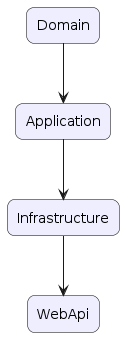
\includegraphics[height=0.75\textheight, keepaspectratio]{references.png}
    \end{minipage}\hfill
    \begin{minipage}{0.45\textwidth}
        \centering
        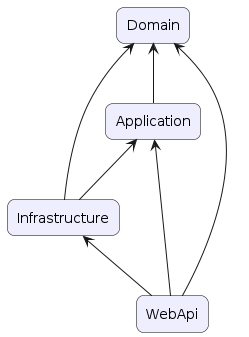
\includegraphics[height=0.75\textheight, keepaspectratio]{visibility.png}
    \end{minipage}
\end{figure}
\end{frame}

\begin{frame}
\frametitle{CQRS}
CQRS (Command Query Responsibility Segregation) is a design pattern that separates reading data (queries) from modifying it (commands). Each type of operation is handled by its own model, which makes the system easier to reason about and maintain.

This separation improves clarity — commands express intent to change state, while queries focus purely on retrieving information.

In Clean Architecture, CQRS fits naturally into the structure of use cases, reinforcing the idea that each action in the application should have a clear and single responsibility. It also enables better scalability and flexibility when evolving the system.
\end{frame}

\begin{frame}
\frametitle{Test-Driven Development}
Test-Driven Development (TDD) is a software development approach where tests are written before the actual implementation. The process follows a short and repeatable cycle: Red → Green → Refactor — first writing a failing test, then implementing the simplest code to make it pass, and finally improving the design while keeping tests green.

TDD encourages clean, modular, and maintainable code by ensuring every piece of functionality is covered by automated tests from the start.

In the context of Clean Architecture, TDD reinforces the separation of concerns — allowing developers to focus on business logic and behavior first, independent of frameworks or infrastructure.
\end{frame}

\begin{frame}
\frametitle{Unit Tests}
Unit Tests in Clean Architecture focus on verifying the core business logic in complete isolation. They test individual classes, methods, or domain rules without involving databases, files, or external services.

These tests live close to the Domain and Application layers, ensuring that business rules and use case logic behave exactly as intended. Because they run fast and are fully deterministic, they provide immediate feedback when something breaks.

Their purpose is to guarantee that the inner layers of the system remain correct and stable, regardless of changes in infrastructure or frameworks — preserving the integrity of the application’s core behavior.
\end{frame}

\begin{frame}
\frametitle{Functional Tests}
Functional Tests in Clean Architecture verify that entire use cases work correctly as a whole — from the application layer through to the infrastructure. They test the system’s behavior from the outside, focusing on what it does rather than how it’s implemented.

These tests often execute real commands and queries against a configured application instance, sometimes using an in-memory or test database.

They validate that the application’s components — handlers, repositories, and domain logic — collaborate correctly to fulfill business requirements, providing strong confidence that the system behaves as expected in real-world scenarios.
\end{frame}

\begin{frame}
\frametitle{End to End Tests}
End-to-End (E2E) Tests in Clean Architecture validate the entire system from the user’s perspective — across all layers, from the presentation interface down to the database and back.

They simulate real workflows, such as API calls or user interactions, ensuring that all components integrate correctly and deliver the expected business outcomes.

E2E tests provide the highest level of confidence that the system functions as a cohesive whole, but they are slower and more complex to maintain, so they are typically reserved for critical paths and key scenarios that must always work end-to-end.
\end{frame}
\end{document}